% LL3M: L3-Resident Ternary Language Model with Host-Side Knowledge
% Draft v0.7.9 -- P1 ablations (gate stats, KB on/off, multi-seed SciQ probe)
% Build: tectonic -X compile ll3m_l3_resident.tex
%    or: pdflatex && bibtex && pdflatex && pdflatex
\documentclass[11pt,a4paper]{article}

\usepackage[margin=1in]{geometry}
\usepackage{times}
\usepackage{amsmath,amssymb,amsthm}
\usepackage{booktabs}
\usepackage{graphicx}
\usepackage{hyperref}
\usepackage{microtype}
\usepackage{xcolor}
\usepackage{enumitem}
\usepackage{caption}
\usepackage{natbib}
\usepackage{url}
\usepackage{float}
\usepackage[section]{placeins}

\hypersetup{
  colorlinks=true,
  linkcolor=blue!50!black,
  citecolor=blue!50!black,
  urlcolor=blue!50!black
}

\graphicspath{{figures/}}

\title{\textbf{LL3M: CCD-Gated Co-Design of a Ternary\\Language Model for One L3 Slice}}
\author{
  Marcel Wysocki
}
\date{Draft v0.7.9 \quad 2026-08-03}

\begin{document}
\maketitle

\begin{abstract}
Most ``small'' LMs still target phones or discrete GPUs with multi-hundred-megabyte payloads.
We ask a different question: \emph{what if the product unit is one CPU last-level cache (L3) CCD?}
\textbf{LL3M} co-designs architecture, ternary/int8 quantization, portable C packing, curriculum, and host memory so the \emph{entire} inference working set (weights + activations + KV) \textbf{size-fits} a single CCD gate ($\sim$30.4\,MiB on a 32\,MiB slice).

The freeze is $\sim$79M parameters (L23$\times$d576 MQA, $T{=}256$, $V{=}2048$), served as a \textbf{20.3\,MiB} \texttt{L3T2} pack with continuous QAT matching C.
\textbf{Knowledge placement} is first-class: ternary weights hold language and tool policy; facts live in a host Engram-lite KB and tools.
On seven zero-shot MC tasks ($n{=}400$, denser-continue pack), macro is \textbf{41.4\%} vs \textbf{54.2\%} for Qwen3.5-0.8B-Base under portable weight-only int4 (\textbf{$-$12.8\,pp} absolute; $\sim$9.5$\times$ more Qwen params; not iso-tokenizer/data).
Tool-only SFT regresses SciQ by 18\,pp; multi-mix SFT restores SciQ (macro 41.2\%).
On a \textbf{closed} 101-case agent suite (not BFCL), the tool-SFT ship pack scores \textbf{90/101 pure} (assist and gate off; no\_call 15/24) and \textbf{101/101 product} only with assist off and a When2Call-style \textbf{host gate on}---product quality is model emission $\times$ host policy, not model-only competence.
Artifact pins: \texttt{checkpoints/paper\_freeze\_v072/} (SHA256 in \texttt{MANIFEST.json}).

On the reference host, C decode \textbf{size-fits} one CCD (runtime WS \textbf{24.3\,MiB}; design \textbf{30.2\,MiB}) with 100\% mlock; hard+FIFO holds $\sim$\textbf{280--282}\,tok/s.
DRAM share of L2 fills is often \textbf{WEAK} without isolation; \textbf{GOOD} ($\le$5\%) appears only under hard+FIFO / quiet-core (preferably \texttt{isolcpus}) paths---not a portable zero-DRAM guarantee.
Multi-session packing under the same size gate reaches $N{=}2$ at full $T$ ($\sim$550 tok/s aggregate) and $N{=}8$ with \textbf{short KV} ($\sim$2100--2200 aggregate).
We \textbf{name and operationalize} \textbf{CCD-gated co-design}: a hard L3 size-fit constraint forcing joint shape/quant/serve/data/host choices, with train--serve lock, honest PMU, and dual product/pure agent metrics.
\end{abstract}

\paragraph{Keywords.}
CCD-gated co-design; L3-resident inference; ternary QAT; knowledge placement; tool-augmented SLMs; cache-first systems.

\begin{figure}[H]
  \centering
  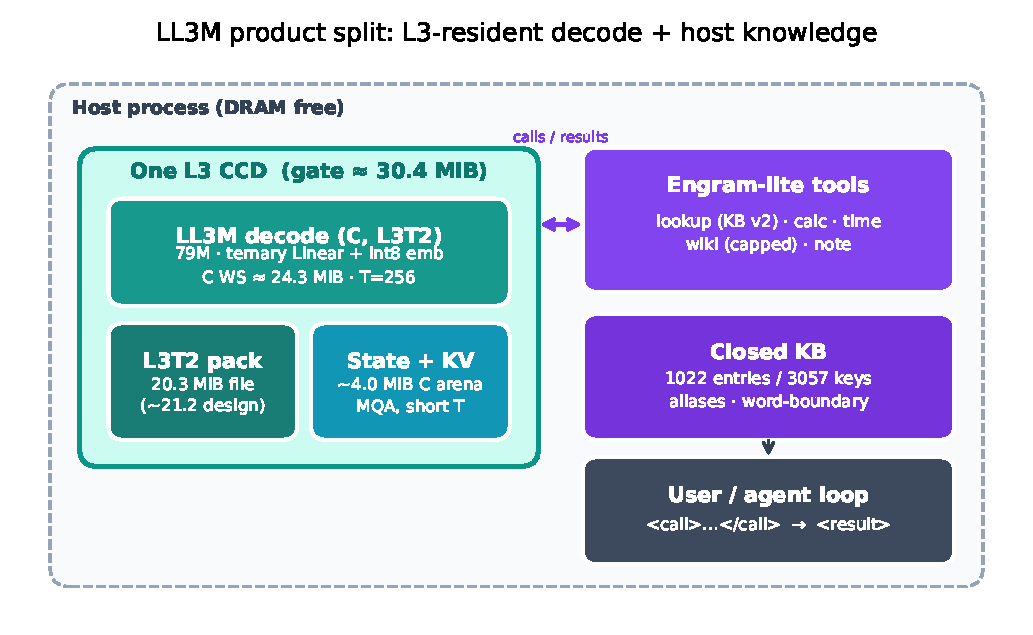
\includegraphics[width=0.98\linewidth]{fig_system_arch.pdf}
  \caption{\textbf{CCD-gated split.} Decode stays inside one L3 CCD (\texttt{L3T2} pack + state/KV); host Engram-lite tools own long-tail facts. C runtime WS $\approx$24.3\,MiB; design estimate $\approx$30.2\,MiB under a 30.4\,MiB gate.}
  \label{fig:arch}
\end{figure}

%----------------------------------------------------------------------
\section{Introduction}
\label{sec:intro}

\paragraph{Objective.}
Most small-LM work optimizes quality under a parameter or memory budget.
We use a stricter unit: \textbf{one CPU L3 CCD}.
If weights, activations, and KV \textbf{size-fit} that slice, residency hooks can keep the hot set off the DRAM path when the host cooperates---orthogonal to FLOP counts and to phone-GPU 4-bit footprints.

\paragraph{Why not just another tiny BitNet.}
Ternary nets~\citep{ma2024bitnet,wang2023bitnet}, educational data~\citep{gunasekar2023textbooks,allal2025smollm},
on-device SLMs~\citep{liu2024mobilellm}, and tool agents~\citep{patil2023gorilla,when2call} each exist.
Missing is an end-to-end \textbf{product freeze} that makes full-decode L3 residency non-negotiable:
MQA at short $T$, tiny BPE, ternary+int8 packs, C residency hooks, host facts, and a dense multi-mix ladder under continuous QAT.

\paragraph{Thesis.}
\begin{quote}
\textit{Under a single-CCD inference gate, capability is maximized by co-designing shape, quant, runtime, data, and host memory---not by packing more facts into ternary weights.}
\end{quote}

\paragraph{Contributions.}
\begin{enumerate}[leftmargin=*,itemsep=1.5pt]
  \item \textbf{CCD gate as objective:} $0.95\times$ one 32\,MiB CCD ($\sim$30.4\,MiB); design WS $\sim$30.22\,MiB; C runtime WS $\sim$24.3\,MiB; on-disk pack 20.3\,MiB for 78\,815\,712 ternary+int8 params (L23$\times$d576 MQA, $T{=}256$, $V{=}2048$).
  \item \textbf{Train--serve quant lock:} continuous ternary Linear + int8 embed QAT; portable C \texttt{L3T2}; residency hooks with measured \textbf{size-fit} and honest PMU (DRAM\% host-dependent).
  \item \textbf{Knowledge placement:} host Engram-lite KB (1022 entries / 3057 keys) + tools for facts; weights for language + tool policy.
  \item \textbf{Dense ladder + dual agent metrics:} tool-only SFT harms SciQ ($-$18\,pp); multi-mix restores SciQ; tool ship is \textbf{90/101 pure} vs \textbf{101/101 product} (host gate on) on a closed suite---not BFCL.
\end{enumerate}

\paragraph{Claim $\rightarrow$ checkpoint map.}
Table~\ref{tab:claimmap} states which pack answers which metric (dual-SKU is intentional).
\begin{table}[H]
\centering
\caption{Which checkpoint answers which claim (v0.7.9).}
\label{tab:claimmap}
\small
\setlength{\tabcolsep}{3pt}
\begin{tabular}{@{}p{0.28\linewidth}p{0.34\linewidth}p{0.30\linewidth}@{}}
\toprule
Claim & Checkpoint / pin & Metric \\
\midrule
Closed-book macro 41.4\% & \texttt{v76\_dense\_c} denser continue & 7-task MC, $n{=}400$ \\
SciQ peak 69.5\% & \texttt{v76\_dense\_c\_p1} (C+) & SciQ / macro flat \\
Tool ship pure 90/101 & \texttt{pure\_v2} + freeze pure pin & assist off, gate off \\
Tool ship product 101/101 & \texttt{pure\_v2} + freeze product pin & assist off, gate on \\
KB snapshot & \texttt{paper\_freeze\_v072/kb\_facts.json} & 1022 / 3057 \\
Size-fit / tok/s & denser-C \texttt{L3T2} on ref.\ host & WS 24.3\,MiB; $\sim$280 tok/s \\
\bottomrule
\end{tabular}
\end{table}

\paragraph{Non-goals.}
We do not claim MMLU parity with 0.5B--8B models, L3-resident training, MoE, pure 1-bit weights, BFCL SOTA, or $\sim$0\% DRAM share without isolation.
We claim a \textbf{measured operating point} under a rare constraint.

%----------------------------------------------------------------------
\section{Positioning}
\label{sec:novelty}

Table~\ref{tab:novelty} states the contribution as a \textbf{conjunction} under a hard CCD gate, not any single brick.

\begin{table}[H]
\centering
\caption{Novelty as constraint-driven conjunction (not isolated algorithms).}
\label{tab:novelty}
\small
\setlength{\tabcolsep}{3.5pt}
\begin{tabular}{@{}p{0.18\linewidth}p{0.24\linewidth}p{0.24\linewidth}p{0.26\linewidth}@{}}
\toprule
Axis & Typical SLM / BitNet & Typical tool agent & \textbf{LL3M (this work)} \\
\midrule
Primary budget & params / VRAM / disk & API / latency & \textbf{one L3 CCD WS} \\
Serve claim & PyTorch / mobile NPU & cloud tools & \textbf{portable C + residency} \\
Quant story & post-hoc or train-only & often fp16 student & \textbf{QAT locked to C pack} \\
Knowledge & more pretrain tokens & RAG/tools add-on & \textbf{placement under gate} \\
Success metric & MMLU-style only & tool accuracy only & \textbf{MC + agent + WS fit} \\
\bottomrule
\end{tabular}
\end{table}

\paragraph{Named principle.}
We \textbf{name and operationalize} \textbf{CCD-gated co-design}: a component is admissible only if the hot WS estimate and C pack respect the CCD gate; knowledge that cannot fit is externalized.
This is a product constraint, not a new attention operator.

%----------------------------------------------------------------------
\section{Related work}
\label{sec:related}

\paragraph{Data-efficient small LMs.}
Phi and SmolLM emphasize educational filtering and synthetic textbooks~\citep{gunasekar2023textbooks,li2023textbooks2,allal2025smollm,penedo2024fineweb,eldan2023tinystories}.
MobileLLM studies sub-billion on-device shapes~\citep{liu2024mobilellm}.
We keep the density intuition but \textbf{subordinate it to a CCD gate}, which forbids large vocabs and long contexts that those lines often retain.

\paragraph{Ternary / 1.58-bit training.}
BitNet b1.58 and bitnet.cpp~\citep{ma2024bitnet,wang2023bitnet,bitnetcpp2025,bitnetcpp} establish ternary STE and packing.
LL3M's incremental systems contribution is \textbf{native QAT through a multi-stage dense ladder} with explicit checkpoint assertions and a C residency path under a fixed WS ceiling.

\paragraph{External memory and tools.}
Engram~\citep{deepseek2026engram} argues for O(1) lookup beside neural compute.
Tool-calling work~\citep{patil2023gorilla,when2call,vanroy2025slmfc,chen2024octopus,lacy2026} shows small models need narrow schemas, gold SFT, and no-call negatives.
We operationalize a lightweight Engram split for a \textbf{79M ternary} model: host KB is mandatory product infrastructure, not an optional RAG demo.

\paragraph{Cache-aware inference.}
Kernel and paging systems~\citep{llamacpp,mlcllm,song2023powerinfer} improve average-case locality.
We instead use a \textbf{hard product refusal}: if estimated WS exceeds the CCD gate, the shape is rejected at design time; we further report measured mlock and PMU on the C path.

%----------------------------------------------------------------------
\section{System design}
\label{sec:system}

\subsection{Architecture}
\label{sec:arch}

\begin{table}[H]
\centering
\caption{LL3M product shape (v2 block).}
\label{tab:shape}
\small
\begin{tabular}{@{}p{0.28\linewidth}p{0.66\linewidth}@{}}
\toprule
Component & Choice \\
\midrule
Block & RMSNorm, RoPE, SwiGLU, QK-Norm, no bias \\
Depth / width & 23 layers, $d{=}576$, mid 1536 \\
Attention & 12 Q / 1 KV (MQA), $d_h{=}48$~\citep{shazeer2019mqa,ainslie2023gqa} \\
Context / vocab & $T{=}256$, BPE $V{=}2048$ \\
Stability & LayerScale $10^{-4}$; peri-LN \textbf{off} \\
Train extras & z-loss~\citep{palm2022}; shared-head MTP~\citep{deepseekv3} (train-only) \\
Parameters & 78\,815\,712 \\
\bottomrule
\end{tabular}
\end{table}

Table~\ref{tab:shape} summarizes the freeze.
At short $T$, MQA cheapens KV so depth/width absorb parameters under the gate.
Peri-LN blocked early learning on this shape (val CE stuck $\sim$5.9 in short ablations); LayerScale alone progressed.

\subsection{Quantization and pack}
\label{sec:quant}

Linear layers use ternary STE (absmean) in train and 2-bit packing in C.
Embeddings use int8 QAT: ternary embeds traded quality for a sub-MiB L3 win in earlier ablations.
Export produces \texttt{.ll3m} (\texttt{L3T2}); denser-C on-disk pack is \textbf{20.32\,MiB} (C weights payload after load: 20.27\,MiB).
Training may use full DRAM/GPU; the product claim is C decode.

\paragraph{Post-hoc vs QAT (v75 lineage).}
Forcing ternary+int8 on an fp32 checkpoint raised val CE from 1.14 to 2.27; native ternary+int8 QAT on the same shape sits near val CE 1.26 on the serve grid.
This supports continuous QAT over naive post-hoc pack.

\paragraph{Portable int4 baseline (Qwen).}
Per-row absmax fake-quant of Linear weights (not NF4, GPTQ, or NVFP4).
For each row~$i$, set $s_i=\max_{j}|w_{ij}|/7$.
Round each scaled entry and clip to $q_{ij}\in\{-8,\dots,7\}$, then set
\begin{equation}
\hat{w}_{ij}=s_i\,q_{ij}.
\end{equation}
See \citet{frantar2023gptq,dettmers2023qlora} for related methods; we use a simpler portable weight-only protocol.

\subsection{L3 residency}
\label{sec:l3}

On the reference host (2$\times$32\,MiB L3 CCD), the product budget is $0.95\times 32\,\mathrm{MiB}\approx 30.4\,\mathrm{MiB}$.
Design-time estimate:
\begin{equation}
  \mathrm{WS}_{\mathrm{design}} \approx W_{\mathrm{weights}} + W_{\mathrm{acts}} + W_{\mathrm{KV}}.
\end{equation}
Design estimator: $\sim$30.22\,MiB (weights $\sim$21.2 + acts/KV $\sim$9.0).
C runtime payload on denser-C: \textbf{24.32\,MiB} (weights 20.27 + state/KV arena 4.00 + pads).
Soft/hard modes include CCD bind, \texttt{mlock}, hierarchical warm, optional isolcpus / FIFO / hugepages.

\begin{figure}[H]
  \centering
  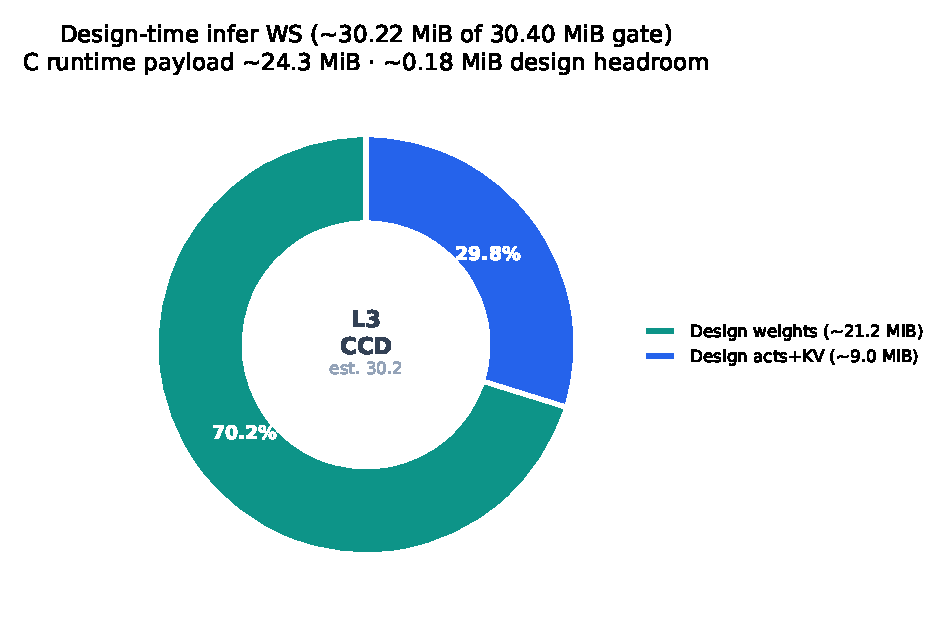
\includegraphics[width=0.72\linewidth]{fig_ws_breakdown.pdf}
  \caption{\textbf{Design-time} inference working-set estimate under the 30.4\,MiB gate (shape freeze). C runtime measures a leaner $\sim$24.3\,MiB payload on the same pack; both fit one 32\,MiB CCD.}
  \label{fig:ws}
\end{figure}

\subsection{Host knowledge (Engram-lite)}
\label{sec:host}

Closed facts live in a JSON KB (v2: canonical ids, aliases, flat index; \textbf{1022} entries / \textbf{3057} keys).
\texttt{lookup} uses word-bounded matching (avoid \texttt{pi}$\subset$\texttt{pizza}).
Open-world queries use capped Wikipedia summaries; arithmetic uses host \texttt{calc}.
The model emits tool-policy tokens; the host executes tools.
Host table growth is free density relative to ternary weight bits.
\textbf{KB on/off (lookup subset, $n{=}20$, pure\_v2 greedy):} full KB $\rightarrow$ 20/20; empty KB $\rightarrow$ 0/20 under both product and pure flags (\texttt{kb\_onoff\_ablation.json})---hits are host memory, not weight knowledge.

%----------------------------------------------------------------------
\section{Training curriculum}
\label{sec:train}

\paragraph{Shape search.}
Exhaustive max-parameter search under the gate with practical head sets yields L23$\times$d576 MQA.

\paragraph{Base English.}
We prefer educational web + dense synthetic cards over TinyStories-primary narrative~\citep{eldan2023tinystories}.
Native ternary (+ int8 embed) QAT is kept on the product path.

\paragraph{Dense knowledge ladder.}
\begin{enumerate}[leftmargin=*,itemsep=1pt]
  \item \textbf{A:} Host KB expand/normalize.
  \item \textbf{B:} $\sim$700M synthetic chars (atomic-biased) + $\sim$500M FineWeb-Edu (doc cap 1200); exact + MinHash near-dedup (Jaccard 0.85); $\sim$\textbf{161M} train tokens after BPE.
  \item \textbf{C:} Continue ternary QAT +30k steps $\rightarrow$ denser continue.
  \item \textbf{C+:} Further +15k dense continue under QAT.
  \item \textbf{D:} Fact Q\&A SFT then tool SFT (QAT on).
  \item \textbf{Mix:} Multi-objective SFT from C: $\sim$50\% dense / 20\% fact / 30\% tool, +5k steps, lr $3{\times}10^{-5}$.
  \item \textbf{Ship tools:} tool-focused SFT lineage (\texttt{pure\_v2}).
\end{enumerate}
Every stage asserts checkpoint tags \texttt{qat=ternary}, \texttt{embed\_qat=int8}.
Dense ladder training primarily on remote CUDA; C residency on the local Ryzen L3 reference machine.

\begin{figure}[H]
  \centering
  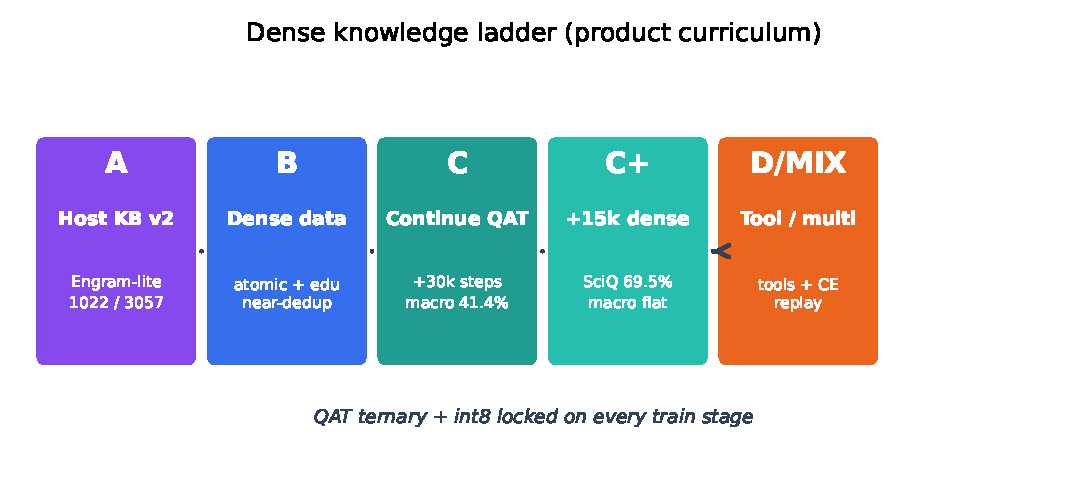
\includegraphics[width=0.90\linewidth]{fig_ladder.pdf}
  \caption{Dense knowledge ladder: host KB $\rightarrow$ atomic/edu data $\rightarrow$ ternary continue $\rightarrow$ C+ $\rightarrow$ tool/multi-mix SFT (QAT locked throughout).}
  \label{fig:ladder}
\end{figure}

\begin{figure}[H]
  \centering
  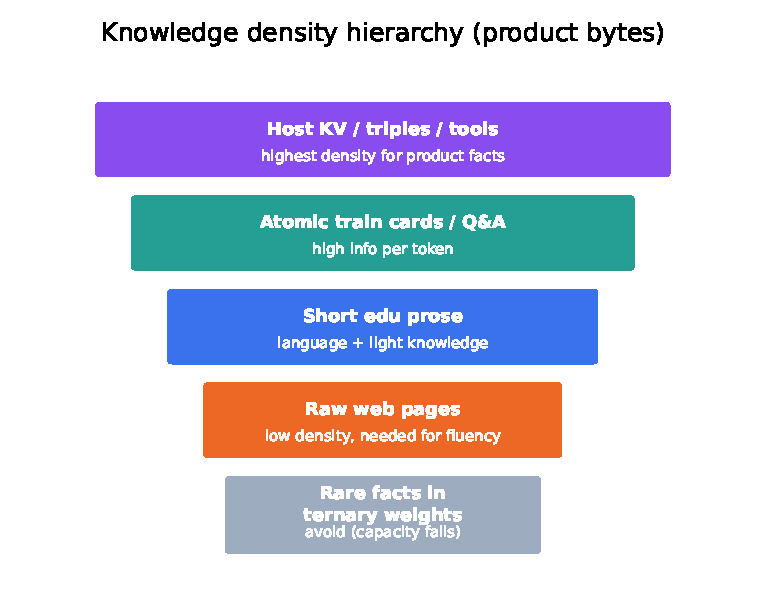
\includegraphics[width=0.62\linewidth]{fig_density_pyramid.pdf}
  \caption{Knowledge density hierarchy for this product: prefer host tables and atomic cards over rare facts in ternary weights.}
  \label{fig:pyramid}
\end{figure}

%----------------------------------------------------------------------
\section{Evaluation}
\label{sec:eval}

\paragraph{MC suite.}
Zero-shot continuation log-likelihood ranking, seed 42, limit 400 examples (COPA uses the full set $n{=}100$):
HellaSwag, ARC-Easy, WinoGrande, BoolQ, OpenBookQA, SciQ, COPA.
Macro accuracy is the unweighted mean of task accuracies.
Domain BPE $V{=}2048$ vs Qwen's large vocab makes this a harsh, not iso-tokenizer, comparison.
Primary tables use seed 42, limit 400.
Bounded multi-seed probe (SciQ only, limit 100, seeds 42/43/44 on denser-C): acc $62/60/60\%$ (mean $60.7\pm 1.2$); paper SciQ 66.5\% is limit 400 seed 42---not interchangeable.

\paragraph{Baseline.}
Qwen3.5 Base family under portable weight-only int4 (equation above), same tasks, limits, and seed.
Primary reference: 0.8B-Base; size ladder also reports 2B/4B/9B.
These are strong industry bases, \emph{not} L3-resident packs.
Canonical compare JSON lives in the repository compare tree (Appendix~\ref{app:artifacts}).

\paragraph{Agent battery.}
Closed suite (101 cases): no-call chat, calc, lookup, time, language openers, adversarial, tokenizer check.
\textbf{Not} BFCL / public When2Call leaderboard.
We always report \textbf{two} flags: \textbf{pure} (assist off, gate off; model-only stress) and \textbf{product} (assist off, gate on; ship = model emission $\times$ host gate).
Gold-inject assist is ablation only.
Decode is C \texttt{L3T2} unless noted.
Primary ship pack is \texttt{pure\_v2}; denser-C pure (42/101) is a language baseline without tool policy.
Pins: Appendix~\ref{app:artifacts} / \texttt{paper\_freeze\_v072/MANIFEST.json}.
Product no-call (24/24) vs pure freeze no-call (15/24) is the main pure$\leftrightarrow$product gap on the ship pin. Gate instrumentation (\S\ref{sec:agent}) logs false-call blocks and tool rewrites; product scores remain \textbf{system} scores.

\paragraph{Residency card.}
C binary with \texttt{{-{-}}l3-resident} / \texttt{{-{-}}residency-hard}, hierarchical warm, CCD bind, optional PMU window after steady-warm.
Logs under \path{checkpoints/compare/}.

%----------------------------------------------------------------------
\section{Results}
\label{sec:results}

\subsection{Closed-book macro}
\label{sec:macro}

\begin{table}[ht]
\centering
\caption{Macro accuracy (7 tasks, $n{=}400$; COPA $n{=}100$). LL3M packs are 20.3\,MiB \texttt{L3T2}. Qwen rows use portable weight-only int4.}
\label{tab:macro}
\begin{tabular}{@{}lrr@{}}
\toprule
Model & Params (approx.) & Macro \\
\midrule
Qwen3.5-0.8B-Base int4 & $\sim$0.75B & \textbf{54.21\%} \\
Qwen3.5-2B-Base int4 & $\sim$1.9B & 59.39\% \\
Qwen3.5-4B-Base int4 & $\sim$4.2B & 64.96\% \\
Qwen3.5-9B-Base int4 & $\sim$9.0B & 69.11\% \\
LL3M prior tool path & $\sim$79M tern. & 40.11\% \\
LL3M denser continue (C) & $\sim$79M tern. & \textbf{41.39\%} \\
LL3M dense continue +15k (C+) & $\sim$79M tern. & 41.36\% \\
LL3M tool/fact SFT (D) & $\sim$79M tern. & 40.46\% \\
LL3M multi-mix SFT (MIX) & $\sim$79M tern. & \textbf{41.18\%} \\
\bottomrule
\end{tabular}
\end{table}

Table~\ref{tab:macro} and Figure~\ref{fig:macro} summarize macros.
\textbf{C vs Qwen 0.8B int4:} \textbf{$-$12.82\,pp absolute} on this suite ($\sim$9.5$\times$ Qwen params; portable absmax int4, not NF4/GPTQ; not iso-tokenizer).
Relative deficit $1-41.39/54.21\approx 23.6\%$ is secondary and easy to over-read as near-parity.
Vs 9B int4 the absolute gap is $-$27.7\,pp.
\textbf{C+} does not lift macro despite SciQ gains (Table~\ref{tab:tasks}).
LL3M remains an L3-class pack (20.3\,MiB) under a CCD gate that the Qwen bases do not target (Figure~\ref{fig:scale}).

\begin{figure}[ht]
  \centering
  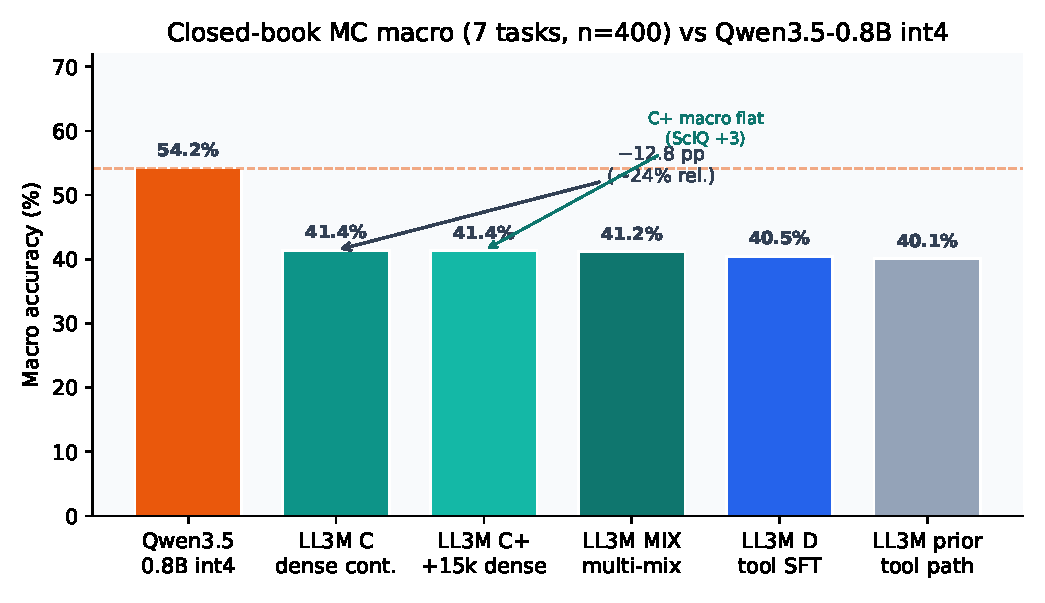
\includegraphics[width=0.92\linewidth]{fig_macro_bars.pdf}
  \caption{Macro accuracy on seven standard MC tasks ($n{=}400$). LL3M denser continue (C) reaches 41.4\% versus 54.2\% for Qwen3.5-0.8B-Base weight-only int4.}
  \label{fig:macro}
\end{figure}

\begin{figure}[ht]
  \centering
  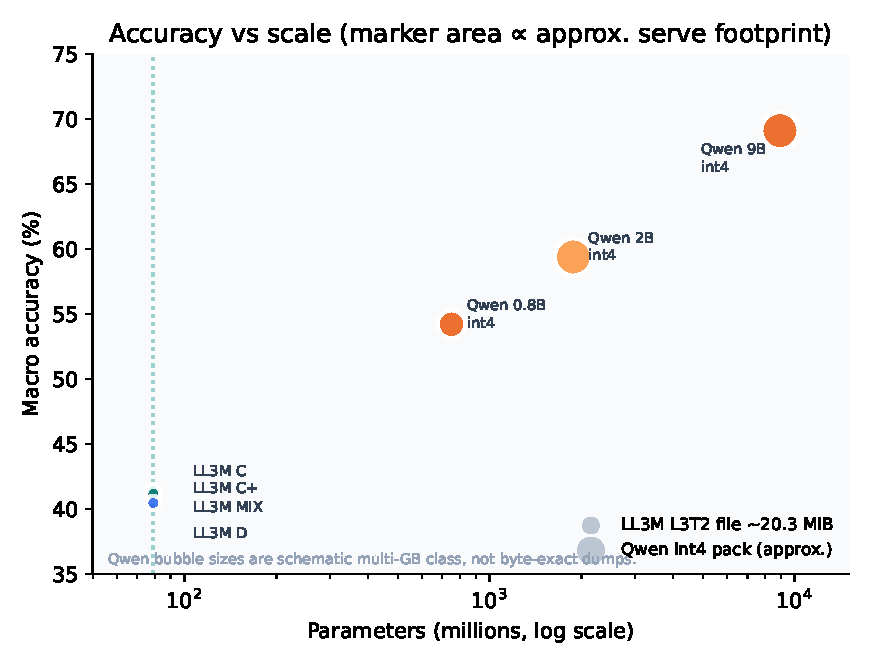
\includegraphics[width=0.82\linewidth]{fig_size_tradeoff.pdf}
  \caption{Accuracy versus parameter scale. Marker area is proportional to approximate serve footprint (LL3M L3T2 file 20.3\,MiB; Qwen bubbles schematic multi-GB class).}
  \label{fig:scale}
\end{figure}

\subsection{Per-task detail}
\label{sec:pertask}

\begin{table}[ht]
\centering
\caption{Per-task accuracy (\%). Qwen column is portable weight-only int4 (macro 54.21\%). Random $\approx$25--50\% depending on the task. COPA $n{=}100$.}
\label{tab:tasks}
\setlength{\tabcolsep}{3.5pt}
\begin{tabular}{@{}lrrrrrr@{}}
\toprule
Task & C & C+ & D & MIX & Qwen 0.8B int4 & Rand. \\
\midrule
HellaSwag & 28.0 & 28.5 & 26.5 & 29.0 & 35.5 & 25 \\
ARC-Easy & 27.3 & \textbf{29.8} & 31.0 & 27.8 & 59.0 & 25 \\
WinoGrande & 47.5 & 48.0 & 51.0 & 50.0 & 49.8 & 50 \\
BoolQ & \textbf{56.0} & 47.8 & 54.3 & 46.5 & 63.0 & 50 \\
OpenBookQA & 13.5 & 13.0 & 16.0 & 12.5 & 21.0 & 25 \\
SciQ & 66.5 & \textbf{69.5} & 48.5 & 66.5 & 84.3 & 25 \\
COPA & 51.0 & 53.0 & 56.0 & 56.0 & 67.0 & 50 \\
\bottomrule
\end{tabular}
\end{table}

Tool-only SFT (D) harms SciQ ($-$18\,pp vs C) while helping some two-way tasks (Figure~\ref{fig:pertask}).
Multi-mix SFT restores SciQ and keeps macro near C: CE replay is required when adding tools at this scale.
Further dense continue (C+) specializes: SciQ $+3.0$ and ARC-Easy $+2.5$, BoolQ $-8.2$, macro flat.
Val CE never beat the C resume bar on C+, yet end-of-run weights improved SciQ (multi-domain best-val is a false friend).

\begin{figure}[ht]
  \centering
  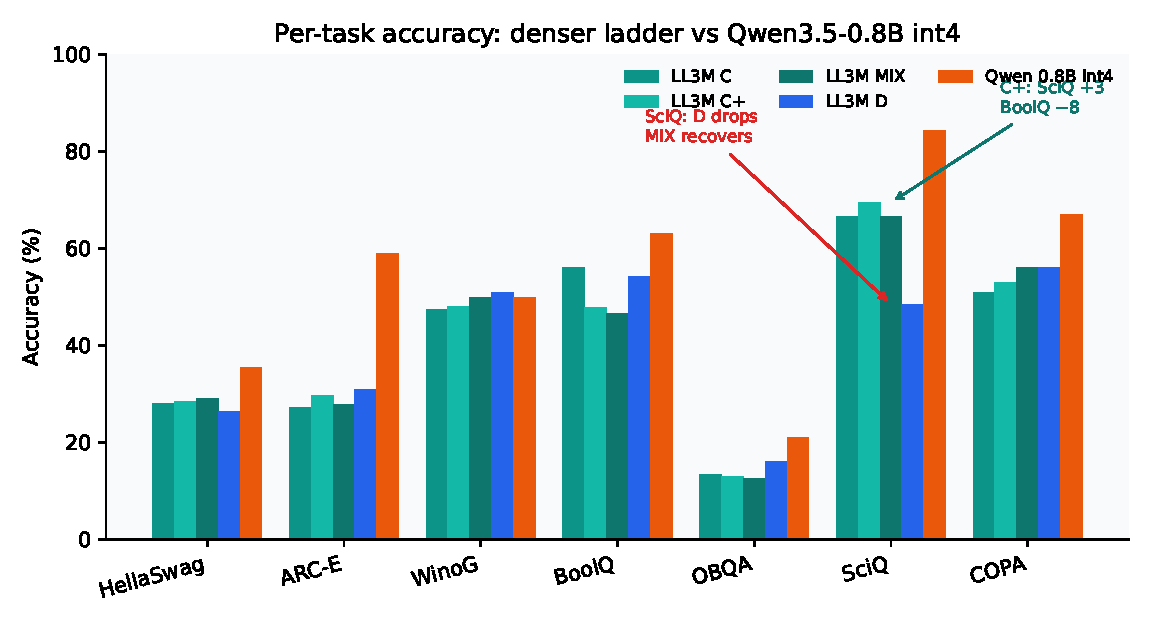
\includegraphics[width=0.95\linewidth]{fig_pertask.pdf}
  \caption{Per-task accuracy including C+. Multi-mix recovers SciQ after tool-only SFT regression while staying near denser-continue macro.}
  \label{fig:pertask}
\end{figure}

\subsection{Agent battery}
\label{sec:agent}

\begin{table}[ht]
\centering
\caption{Closed 101-case agent battery (C \texttt{L3T2}, greedy). Product = assist off, host gate on.}
\label{tab:agent}
\setlength{\tabcolsep}{3.5pt}
\begin{tabular}{@{}llrrrr@{}}
\toprule
Lineage & Policy & Total & calc & lookup & no\_call \\
\midrule
pure\_v2 & product & \textbf{101/101} & 30/30 & 20/20 & 24/24 \\
pure\_v2 & pure & \textbf{90/101} & 30/30 & 20/20 & 15/24 \\
denser C & pure & 42/101 & 0/30 & 0/20 & 24/24 \\
D & pure & 37/101 & 3/30 & 7/20 & 8/24 \\
MIX & pure & 70/101 & 24/30 & 19/20 & 2/24 \\
\bottomrule
\end{tabular}
\end{table}

Table~\ref{tab:agent} uses tool-SFT ship weights (\texttt{pure\_v2}).
\textbf{Read pure first:} freeze pure is 90/101 with no\_call 15/24 (stream-visible scoring on the ship pin).
\textbf{Product 101/101} is a \textbf{system} score (assist off, host gate on).

\paragraph{Gate decomposition (instrumented re-run).}
On the same pure\_v2 pack with host-gate event logging (\texttt{battery\_*\_gatestats.json}):
\begin{itemize}[leftmargin=*,itemsep=1pt]
  \item Agent protocol cases: 85 (of 101 total with host/lang/tok checks).
  \item Model emitted a parseable \texttt{<call>} on \textbf{85/85} protocol cases.
  \item Gold host intent needs a tool on 58 cases; the model called on \textbf{58/58} (0 silent).
  \item On 27 no-tool-intent cases the model still called; with gate on, the host \textbf{blocked all 27} (product no\_call stays 24/24).
  \item Host rewrote a wrong tool name to gold intent \textbf{2} times.
  \item With gate off, the same 27 false-call emissions are not blocked: emission-aware pure is \textbf{72/101}; final-text-only recovery is 99/101.
\end{itemize}
Thus product no-call is primarily a \textbf{host gate} result (\S\ref{sec:pareto}); the freeze pure pin (90/101) sits between emission-aware and final-text-only pure.
A prior same-flag product re-run scored 99/101 (2/5 \texttt{time}); pins under \texttt{paper\_freeze\_v072/}.
Suite schema: \texttt{docs/AGENT\_BATTERY\_SUITE.md}.
Train--serve greedy match on the tool ship pack: \textbf{16/16} tokens (C golden).

\subsection{Policy--knowledge Pareto}
\label{sec:pareto}

Short tool-heavy QAT hits a false-call basin (Table~\ref{tab:pareto}).
Denominators shown; SciQ for d12/s2 from SciQ-only runs (same seed/limit).

\begin{table}[ht]
\centering
\caption{Gate-off pure policy vs SciQ under short QAT (denominators explicit).}
\label{tab:pareto}
\setlength{\tabcolsep}{3pt}
\begin{tabular}{@{}lrrrrr@{}}
\toprule
Lineage & calc & lookup & SciQ & no\_call & Note \\
\midrule
denser C & 0/30 & 0/20 & 66.5 & 24/24 & no tools \\
pure\_v2 & 30/30 & 20/20 & 57.75 & 15/24 & ship \\
sciq\_trade & 14/30 & 14/20 & 67.25 & 9/24 & SciQ twin \\
C+ & --- & --- & 69.5 & --- & SciQ peak \\
d12 flood & 30/30 & 20/20 & 60.3 & 7/24 & overtool \\
s2 & 27/30 & 19/20 & 65.8 & 8/24 & SciQ$\to$tools \\
MIX & 24/30 & 19/20 & 66.5 & 2/24 & CE replay \\
\bottomrule
\end{tabular}
\end{table}

\noindent\textbf{Implication.}
Dual ship (agent pack + SciQ/weight twin) and/or product gate are design outcomes under the CCD budget, not temporary engineering debt.
Recovering pure no-call after tool-mass collapse is hard with CE alone.

\paragraph{Preference follow-up (P3).}
Naive DPO on false\_call pairs (1k steps) reaches pure no\_call 24/24 but destroys tools and fluency.
Careful DPO (150 steps, $\sim$55\% tool CE retain, low $\beta$) raises pure total $90{\to}93/101$ (no\_call 23/24) while product gate-on remains strongest on pure\_v2 (\textbf{101/101}).
Product no-call is therefore primarily a \textbf{host gate} result; pure no-call is a research ceiling near the mid-90s without a better multi-objective preference recipe.

\subsection{Residency}
\label{sec:res}

\begin{figure}[H]
  \centering
  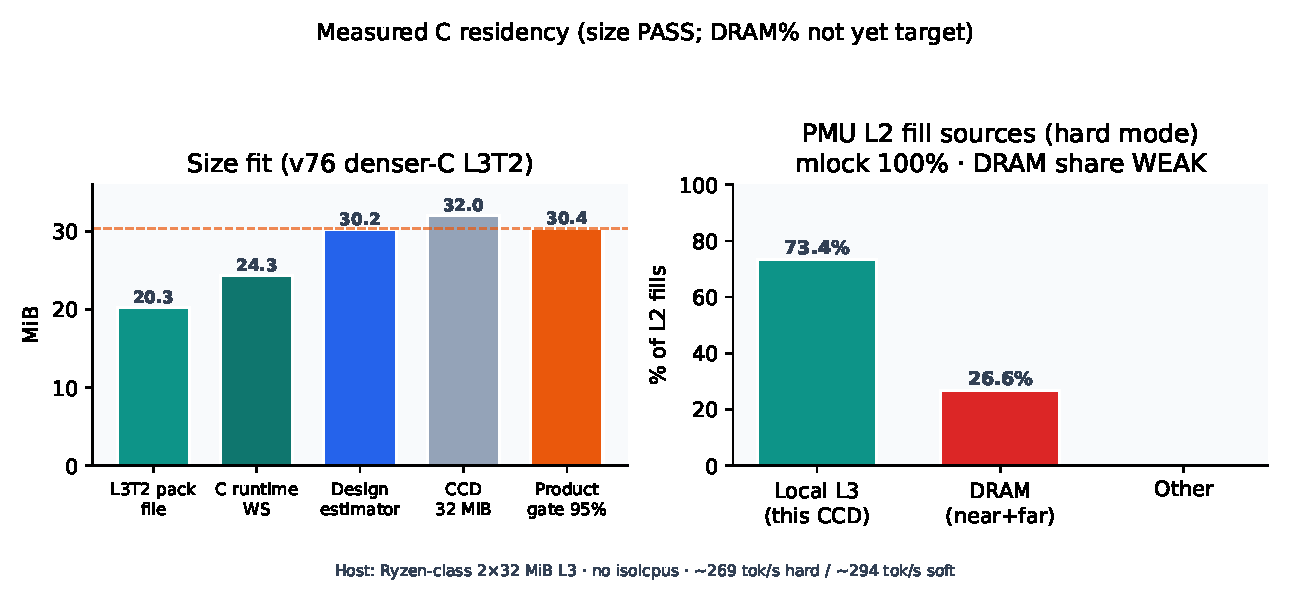
\includegraphics[width=0.96\linewidth]{fig_residency_pmu.pdf}
  \caption{Measured C residency on denser-C \texttt{L3T2}: size-fit PASS (runtime WS 24.3\,MiB $<$ 32\,MiB CCD), mlock 100\%, hard+FIFO can reach GOOD DRAM\% ($\le$5\%) on long windows; soft multi-core is not faster.}
  \label{fig:resid}
\end{figure}

\begin{table}[H]
\centering
\caption{On-host C decode measurement (denser-C pack, reference Ryzen 2$\times$32\,MiB L3).}
\label{tab:resid}
\small
\setlength{\tabcolsep}{4pt}
\begin{tabular}{@{}lrr@{}}
\toprule
Metric & Soft & Hard \\
\midrule
C runtime WS (MiB) & 24.32 & 24.32 \\
L3T2 weights payload (MiB) & 20.27 & 20.27 \\
L3T2 on-disk file (MiB) & 20.32 & 20.32 \\
Fits 32\,MiB CCD & yes & yes \\
mincore mlock & 100\% & 100\% \\
tok/s (preferred) & $\sim$260--270 & $\sim$280--282 \\
Best hard L3 share of L2 fills & --- & up to $\sim$97\% \\
DRAM share of L2 fills & $\sim$30--40\% often & $\le$5\% GOOD / WEAK \\
SCHED\_FIFO & no & OK (\texttt{cap\_sys\_nice}) \\
\bottomrule
\end{tabular}
\end{table}

Table~\ref{tab:resid} and Figure~\ref{fig:resid}: size-fit and mlock hold; hard+FIFO is preferred once \texttt{cap\_sys\_nice} is available.
Boot \texttt{isolcpus} remains the path to more reliable near-zero DRAM.

\paragraph{Multi-session under the same gate.}
Shared weights and independent states obey $WS = W + N\cdot S(\texttt{kv\_cap})$.
Full $T{=}256$ admits $N{=}2$ ($\sim$550 tok/s aggregate); $N{=}3$ is refused.
With shorter KV, $N{=}8$ at $\texttt{kv\_cap}{=}64$--$128$ reaches $\sim$2100--2200 aggregate; $N{=}16$ short-KV peaks $\sim$2300 aggregate (Table~\ref{tab:multi}).

\begin{table}[H]
\centering
\caption{Multi-session packing under the 30.4\,MiB CCD gate (shared L3T2 weights).}
\label{tab:multi}
\small
\begin{tabular}{@{}lrrr@{}}
\toprule
Config & WS (MiB) & tok/s / stream & Aggregate \\
\midrule
$N{=}1$, kv 256 & 24.3 & $\sim$280 & $\sim$280 \\
$N{=}2$, kv 256 (max full $T$) & 28.4 & $\sim$274 & $\sim$550 \\
$N{=}3$, kv 256 & 32.4 & --- & refused \\
$N{=}8$, kv 128 & 29.6 & $\sim$270 & $\sim$2100 \\
$N{=}8$, kv 64 (best balanced) & 25.2 & $\sim$277 & $\sim$2190 \\
$N{=}16$, kv 32--48 (peak agg.) & $\sim$26--28 & $\sim$146 & $\sim$2300 \\
\bottomrule
\end{tabular}
\end{table}

\FloatBarrier
%----------------------------------------------------------------------
\section{Discussion}
\label{sec:disc}

The \textbf{$-$12.8\,pp} closed-book gap vs Qwen3.5-0.8B portable weight-only int4 is largely the \textbf{price of the CCD gate} (plus less data and a tiny vocab).
The relevant metric is quality \emph{per CCD-resident MiB} and agent reliability under host tools, not iso-param MMLU.

Tool-only SFT under a tiny ternary student overwrites educational surface statistics (SciQ $-$18\,pp; pure agent 37/101).
Multi-mix SFT restoring SciQ is systems evidence that \textbf{policy learning must share bandwidth with dense CE} when capacity is CCD-bounded.
Figure~\ref{fig:pyramid} is the knowledge-placement decision procedure when the gate is full.

We separate six budgets: train scale, pack file size, infer WS (design vs runtime), PMU DRAM share, agent policy flags, and multi-session $N$.
CCD-gated co-design forces that distinction.
Future work: \texttt{isolcpus}-grade DRAM\%, same-shape fp32 MC, bitnet.cpp/llama.cpp latency peers, full multi-seed macro grids (SciQ limit-100 probe only so far), and multi-objective preference learning under QAT. KB on/off for lookup is measured (20/20$\to$0/20).

%----------------------------------------------------------------------
\section{Limitations}
\label{sec:limits}

Closed-book MC is not the product objective; $T{=}256$ and $V{=}2048$ limit long documents; LL ranking vs Qwen is not iso-tokenizer.
We did not run multi-trillion-token overtraining or full teacher KD.
Qwen comparisons are iso-task under weight-only int4, not iso-data; NF4 and public $\sim$100M SLMs are absent.
Residency with isolcpus is host-dependent; without it DRAM\% is often WEAK even when size-fit passes.
The agent suite is closed (101 cases), not BFCL; product scores include the host gate.
No pure-policy pack jointly maximizes tools, SciQ, and pure no-call under short QAT.
Primary MC is single-seed limit 400; a SciQ limit-100 three-seed probe has stdev $\sim$1.2 pp. Incomplete GPU-hour ledger; design vs runtime WS differ (both fit the gate).

\FloatBarrier
%----------------------------------------------------------------------
\section{Conclusion}
\label{sec:conc}

We \textbf{named and operationalized} \textbf{CCD-gated co-design}: treat one CPU L3 CCD as the product unit and jointly choose shape, ternary/int8 QAT, C packing, dense data, and host Engram-lite knowledge so the full decode WS \textbf{size-fits}.
LL3M is a concrete operating point ($\sim$79M, 20.3\,MiB pack, design WS $\sim$30.2\,MiB, runtime WS $\sim$24.3\,MiB) with continuous train--serve lock.
Closed-book macro trails Qwen3.5-0.8B portable weight-only int4 by \textbf{$-$12.8\,pp absolute} on this suite while remaining CCD-gated; multi-mix SFT preserves science signal that tool-only SFT destroys.
On the tool ship pack, report \textbf{pure 90/101} and \textbf{product 101/101} (host gate on) as dual metrics on a closed suite---not BFCL.
Size-fit and mlock are measured on the reference host; hard+FIFO holds $\sim$280--282\,tok/s; DRAM\% is often WEAK without isolation.
Multi-session packing reaches $\sim$2k aggregate tok/s at $N{=}8$ \textbf{short KV}.
The path forward is host KB growth, gate-intervention instrumentation, multi-mix or preference learning, multi-session serving, and isolcpus-grade residency---not encyclopedias in ternary weights.

%----------------------------------------------------------------------
\section*{Ethics statement}
A $\sim$20\,MiB pack enables offline CPU use (privacy, edge) and unsupervised local generation.
Closed tools and host gates limit open-ended tool abuse; data licenses and a model card will accompany any public release.

\section*{Reproducibility}
Artifacts are listed in Appendix~\ref{app:artifacts}.
Train used remote CUDA; serve claims target portable C on the L3 reference host.
Reproduce agent scores from \texttt{checkpoints/paper\_freeze\_v072/} (SHA256 in \texttt{MANIFEST.json}).

\section*{Author}
Marcel Wysocki (sole author).

%----------------------------------------------------------------------
\appendix
\section{Hyperparameters}
\label{app:hp}

\paragraph{Dense continue (C).}
Resume ternary base step 60k; absolute steps 90k; Lion; lr $10^{-4}$, warmup 500; microbatch $8\times$ accum 8 (16\,384 tok/step); dropout 0.1; CUDA train.

\paragraph{Multi-mix SFT.}
From C; +5k steps; lr $3{\times}10^{-5}$; mix $\approx$50/20/30 dense/fact/tool by character budget; QAT ternary+int8.

\section{Artifact paths}
\label{app:artifacts}

{\small
\setlength{\tabcolsep}{3pt}
\begin{tabular}{@{}p{0.32\linewidth}p{0.62\linewidth}@{}}
\toprule
Artifact & Path \\
\midrule
Shape freeze & \texttt{checkpoints/v75\_freeze.json} \\
Paper freeze (KB + agent) & \texttt{checkpoints/paper\_freeze\_v072/} (see \texttt{MANIFEST.json} SHA256) \\
Ladder / residency docs & \texttt{docs/DENSE\_*}, \texttt{docs/L3\_RESIDENCY.md} \\
MC JSON (C / C+ / D / MIX) & \texttt{checkpoints/v76\_dense\_*} \\
Qwen int4 aggregate & \texttt{checkpoints/compare/ll3m\_vs\_qwen35\_family\_int4.json} \\
Residency + multi-session & \texttt{checkpoints/compare/} \\
Multi-stream binary & \texttt{c\_infer/multi\_bench} \\
QAT vs post-hoc & \texttt{checkpoints/v75\_ternary/quality\_compare.json} \\
C runtime & \texttt{c\_infer/} \\
Markdown working draft & \texttt{docs/paper/LL3M\_L3\_Resident\_Ternary\_SLM.md} \\
\bottomrule
\end{tabular}
}

%----------------------------------------------------------------------
\bibliographystyle{plainnat}
\bibliography{ll3m_l3_resident}

\end{document}
